% exercise sheet with header on every page for math or close subjects
\documentclass[12pt]{article}
\usepackage[utf8]{inputenc}
\usepackage{latexsym}
\usepackage{multicol}
\usepackage{fancyhdr}
\usepackage{amsfonts}
\usepackage{amsmath}
\usepackage{amssymb}
\usepackage{enumerate}
\usepackage{listings}
\usepackage{graphicx}
\usepackage{amssymb}

% Shortcuts for bb, frak and cal letters
\newcommand{\E}{\mathbb{E}}
\newcommand{\V}{\mathbb{V}}
\renewcommand{\P}{\mathbb{P}}
\newcommand{\N}{\mathbb{N}}
\newcommand{\R}{\mathbb{R}}
\newcommand{\C}{\mathbb{C}}
\newcommand{\Z}{\mathbb{Z}}
\newcommand{\Pfrak}{\mathfrak{P}}
\newcommand{\Pfrac}{\mathfrak{P}}
\newcommand{\Bfrac}{\mathfrak{P}}
\newcommand{\Bfrak}{\mathfrak{B}}
\newcommand{\Fcal}{\mathcal{F}}
\newcommand{\Ycal}{\mathcal{Y}}
\newcommand{\Bcal}{\mathcal{B}}
\newcommand{\Acal}{\mathcal{A}}

% formating
\topmargin -3.5cm
\textheight 22cm
\textwidth 16.0 cm
\oddsidemargin -0.1cm

% Fancy Header on every Page
\pagestyle{fancy}
\lhead{\textbf{Embedded Systems Milestone 1}}
\rhead{Daniel Schäfer (2549458)\\ Rafael Dewes (2548365)\\ Kevin M\"uller (2550062)}
\renewcommand{\headrulewidth}{1.2pt}
\setlength{\headheight}{110pt}

\begin{document}
\pagenumbering{gobble}
\lstset{language=C++}

\section*{Monitor}
\begin{enumerate}
	\item The Scout should at some point in time send a harvesting
position to the Collector.
	\begin{itemize}
		\item \textbf{LTL:} $\mathbf{F}($sendHarvest$)$
		\item \textbf{Not Safety:} There is no bad prexif because for every infinite trace that is not in L we can always append $\{\text{sendHarvest}\}$. This would then be a good prefix. $\emptyset ^{\omega}$ does not have a bad prefix
		\item \textbf{Co-Safety:} Every trace in L has sendHarvest at some point which is a good prefix.
		\item \textbf{Monitorable:} Every finite trace can be extended to a good prefix by appending $\{\text{sendHarvest}\}$ so we do not have an ugly prefix.
		\item \textbf{Automaton:}\\
			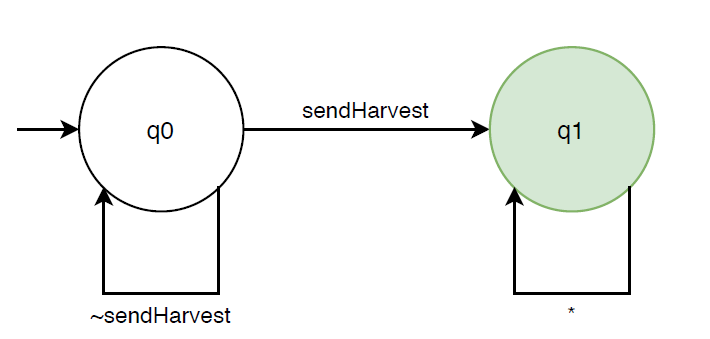
\includegraphics[scale = 0.5]{images/sendHarvestAutomaton}	
		\end{itemize}

\item The Collector should always check its proximity sensors unless it is at a decent harvesting position.
	\begin{itemize}
		\item \textbf{LTL:} $\mathbf{G}(\text{atHarvest} \lor \text{checkingProximity})$
		\item \textbf{Safety:} Every trace not in L has at least one prefix \\
		$\{ \sim \text{atHarvest}  \implies \neg \text{checkingProximity}\}$ which is a bad prefix.
		\item \textbf{Not Co-Safety:} $\{ \text{atHarvest, checkProximity}\}^ {\omega}$ does not have a good prefix. Every trace that is in L does not have a good prefix because we can always do $\{ \neg \text{atHarvest}  \land \neg \text{checkingProximity}\}$ in the next step.
		\item \textbf{Monitorable:} Every finite trace can be extended to a bad prefix so it does not have an ugly prefix.
		\item \textbf{Automaton:} \\
			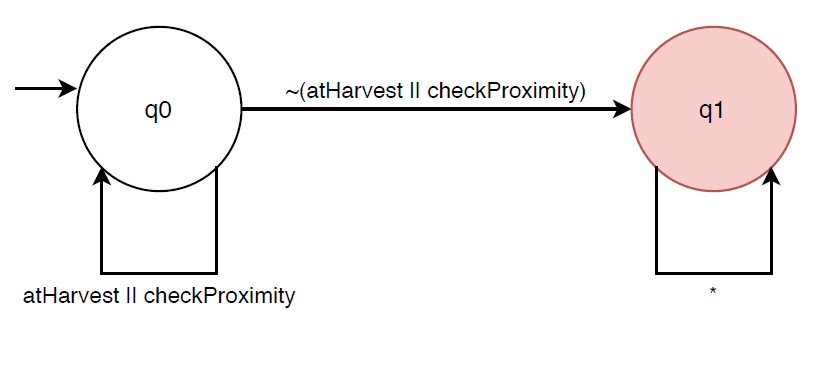
\includegraphics[scale = 0.5]{images/checkProximityAutomaton}
	\end{itemize}		
	
\item A robot should never ignore three consecutive PING messages.
	\begin{itemize}
		\item \textbf{LTL:} $\mathbf{G}((\text{ping} \land \mathbf{X}(\neg \text{pong} \land \text{ping}) \land \mathbf{X}\mathbf{X}(\neg \text{pong} \land \text{ping})) \rightarrow \mathbf{X}\mathbf{X}\mathbf{X} \: \text{pong})$
		\item \textbf{Safety:} Every trace not in L has at least one prefix x which is a bad prefix.
		\item \textbf{Not Co-Safety:} $\{ \text{pong}\}^ {\omega}$ does not have a good prefix. We can extend every good trace to a bad trace by appending $\{\text{ping, ping, ping, ping}\}$.
		\item \textbf{Monitorable:} Every finite trace can be extended with the finite trace $\{\text{ping, ping, ping, ping}\}$ to a bad prefix, therefore we do not have an ugly prefix.
		\item \textbf{Automaton:} \\
			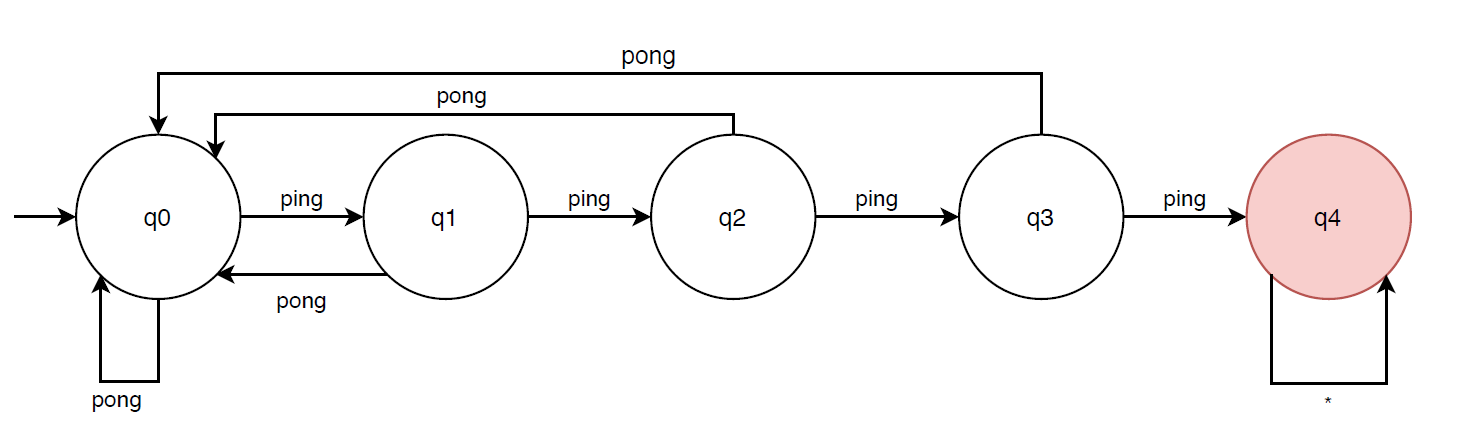
\includegraphics[scale = 0.5]{images/pingAutomaton}
	\end{itemize}		
	
\item When receiving a message, the robot copies the data over into a buffer. This buffer should be emptied at least every 500ms.
	\begin{itemize}
		\item \textbf{LTL:} This specification cannot be expressed in LTL but only in TLTL.
		\item \textbf{Safety:} Every trace not in L has at least one prefix where the buffer is not emptied for more than 500ms, which is a bad prefix.
		\item \textbf{Not Co-Safety:} $\{( \text{emptyBuffer}, t)\}^ {\omega}$ does not have a good prefix for all $t \in \mathbb{N}$ with $0 \leq t \leq 500$. We can extend every such good trace to a bad trace by appending $\{( \text{emptyBuffer}, t + 501)\}$.
		\item \textbf{Monitorable:} Every finite trace be extended to a bad prefix, therefore we do not have an ugly prefix.
		\item \textbf{Automaton:} \\
			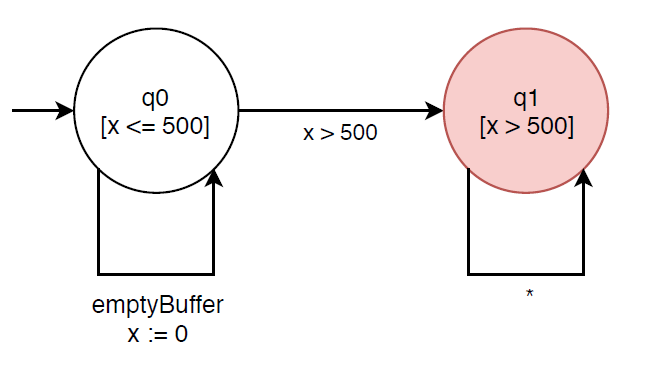
\includegraphics[scale = 0.5]{images/bufferAutomaton}
	\end{itemize}				

\end{enumerate}

\end{document}
